%how to include pdf files in the appendix:
%\cleardoublepage
%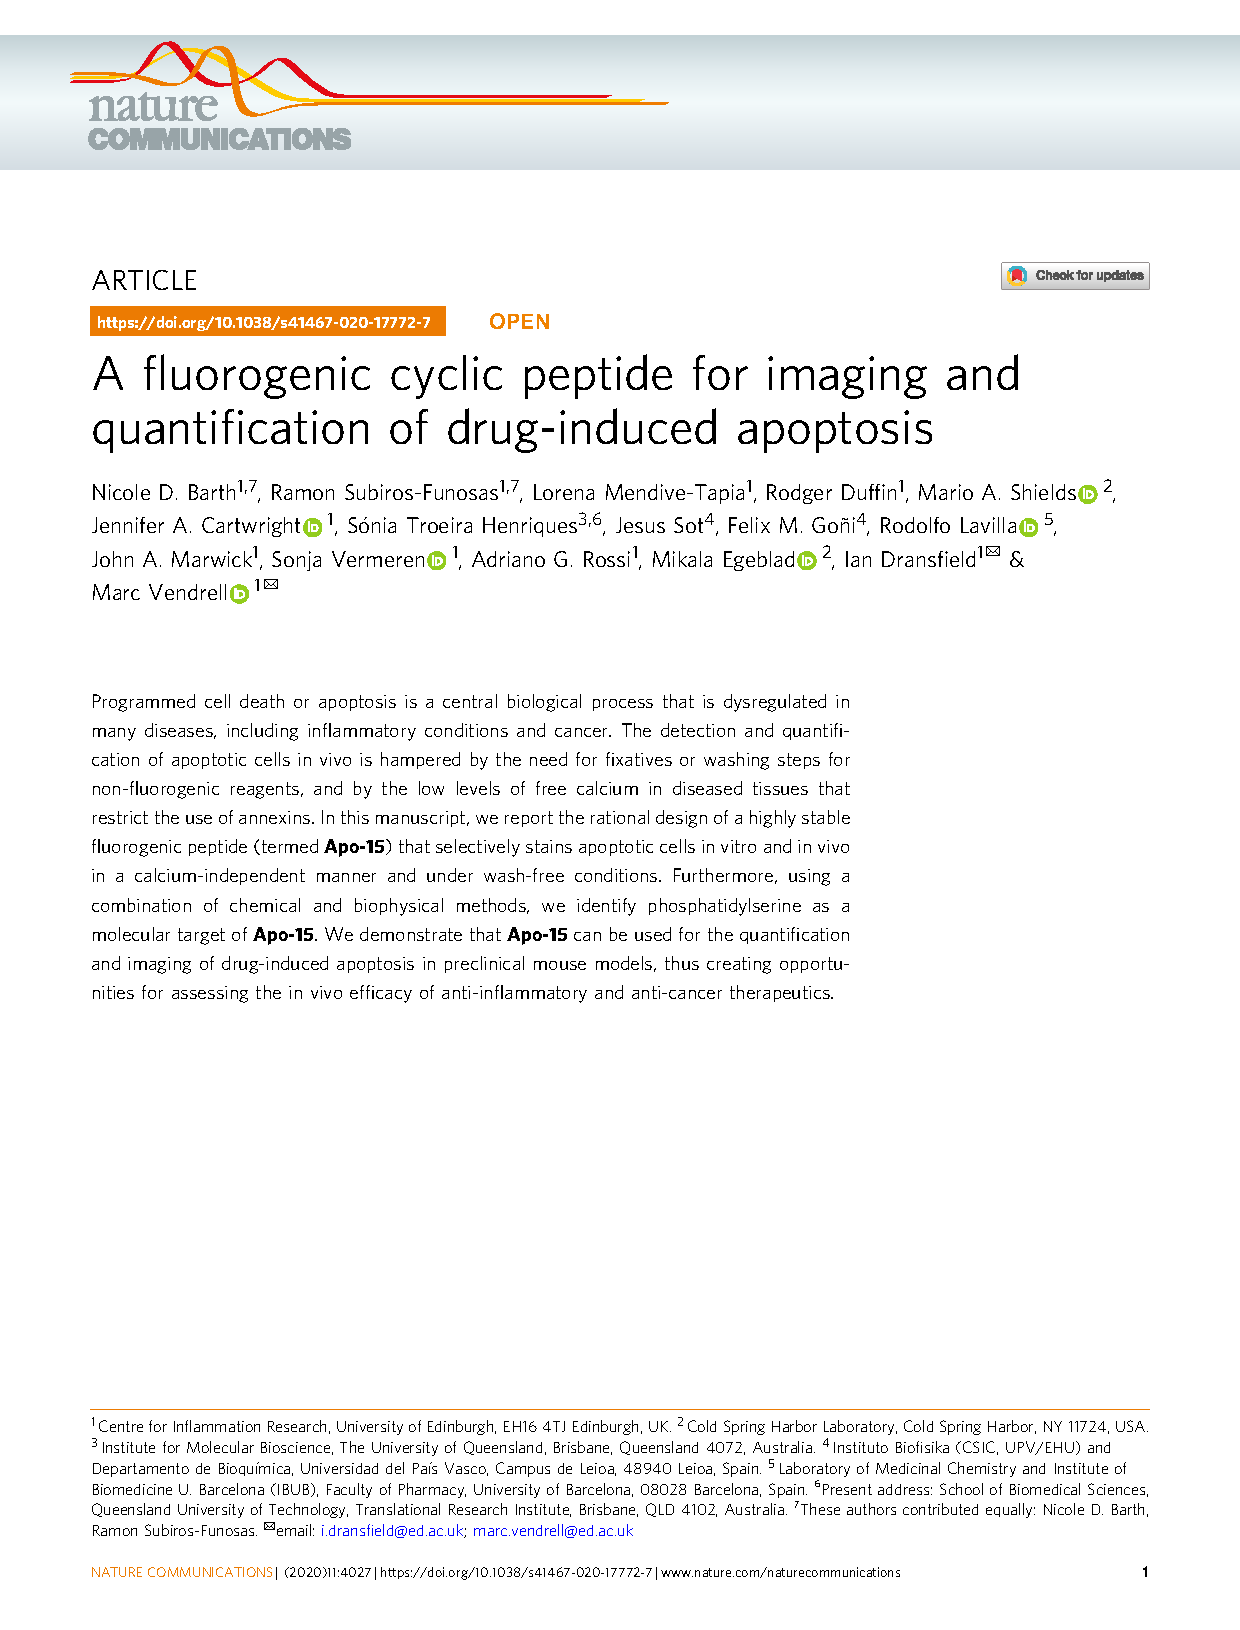
\includepdf[pages=1-2]{appendices/apdfexample.pdf}


%%%%%%%% how to include a note on the bottom of a table in small writing ##########
		%\bottomrule
		%\multicolumn{6}{c}{\footnotesize * Ethanol concentration is above... etc.}
	%\end{tabular}

 ...of aggregation as the sole mechanism causing hemocyte counts to decline with time - 


 To test our experimental assumption, two samples from each group were moderately shaken after the last count, such that any free sedimented hemocytes would be resuspended. The samples were rerun directly after. This measure did not increase the number of singlet hemocytes suspended in MAS or ACB, while those in HLS further decreased (data not shown). This suggests that sedimentation is either preceded by irreversible aggregation, or that hemocytes aggregate irreversibly upon sedimentation. 

hich ruled out sedimentation as an important mechani. sm. Hemocytes did sediment with time, but this was Being the only other conceivable mechanism involved, the assumption was regarded as valid under the current experimental conditions.


Aspirate two samples from the same mussel using different buffers to confirm that the hemocyte medium in fact does not change the SSC vs. FSC profiles of the hemocyte subpopulations within 15 minute incubation. Maybe use crude hemolymph as control?
 

Report pH and osmolarity of the MAS and ACB buffer, and say that it is similar to the osmolarity of hemolymph/seawater 990 mOsm (Hartl, 2010).
- The osmolarity of MAS and ACB were adjusted to approximately 990 mOsm by the addition of \ce{NaCl}, to reflect that of \emph{M. edulis} hemolymph (Hartl, 2010)
- This could be co-presented with the fact that cells did not swell during the incubation period, deducted form the fact that the mean FCS-A did not change.

Aggregation can obscure cell type identification and the counting of single haemocytes, such that clumped haemocytes cannot be included in differentials. In addition, clumping seemed to be more severe among basophillic haemocytes, such that an exclusion of clumped haemocytes could potentially skew the differential. To bypass this problem, haemolymph was withdrawn into an equal volume of 5 \% formaldehyde in MPSS, and fixed in suspension for 1 hour. 

 On the basis of the morphological criteria in section \ref{subsection:morph}, the haemocytes where placed in one of three categories: (1) eosinophilic granulocytes, (2) basophilic granulocytes or (3) small blast-like basophils. 


%                            LABORATORY INSTRUMENTS AND SPECS

BD Accuri C6 Plus benchtop flow cytometer (BD Nordics (prev. Puls Norway), Norway). Filters and lasers.
CytoSub submersible flow cytometer (CytoBuoy, Netherlands)
Coulter Counter Multisizer4 (Beckman Coulter, US) eqipped with a 100 \micro m aperture (size-range 2-60 \micro m)

Nikon Eclipse Ni-U
- Semrock Brightline GFP-4050B filter-cube
- Semrock Brightline LED-Cy5-A
- Plan Fluor 40x/0.75 water immersion objective,
- Plan Fluor 100x/1.30 Oil immersion objective

Nikon Eclipse 90i
- Filter specs?
- Nikon Plan Apo 60XA/1.40 Oil immersion objectice
- Nikon Plan Apo VC 100X/1.40 Oil immersion objective

Leitz Labrolux 12 binocular microscope (Leica Mikroskopi AS, Norway) [EF 40/0.65 objective]
Eppendorf Centrifuge 5804 R (Eppendorf, Norway), [rotor: A-4-44, rotor radius: 15.5 cm], high-speed refrigerated benchtop centrifuge
Jouan KR22i floor centrifuge (Thermo Fischer Scientific, US), high-speed high capacity refrigerated floor centrifuge 8 [rotor: AK 100-21] angle?
Bürker Counting Chamber (Hirschmann Laborgeräte, Germany) with 0.1 mm depth of chamber
Eirik Lund sitt kamera, lense og imaging software: 
Sony ILCE A6400 with E-mount, lense: Tamron 17-70mm F/2.8 
Adobe\textsuperscript{\textregistered} Lightroom Classic 12.0 
BD Microlance$^{TM}$ 3, 23G x 1" - Nr. 16, 0.6mm x 25 mm, sterile, REF 300800
HENKE-JECT 1 mL syringes, 1mL, luer, REF 8300014579, HENKE SASS WOLF GmbH, Tuttlingen, Germany

Since no single experiment would convey the amount of variation observed, no experiments were dedicated to characterize the subpopulations quantitatively. A quantitative approach would nor be especially interesting in itself, since the relative units of FSC and SSC vary heavily between instruments and with instrument settings. The exact light-scatter values are only meaningful when measured on the same instrument, and the insights gained from such measurements are mainly pertained to the relative light-scatter profiles of the different subpopulations.

The deviance-based R$^{2}$ is calculated to according to equation to: $R^{2} = 1 \dfrac{Residual ~ deviance}{Null ~ deviance}$. The adjusted deviance-based R$^{2}$ is calculated according to: $Adjusted ~ R^{2} = 1 - \dfrac{n-1}{n-p}(1 - R^{2})$. This was done using the \emph{adjR2()} function of the \emph{glmtoolbox} in RStudio (\cite{RStudio}).

\begin{table}[H]
	\centering
	\caption{Parameter estimates with 95\% CI, Wald z-values and the belonging p-value are presented for the fitted mixed logistic regression model presented in result section \ref{section:Results_Method_Development}.}
	\label{tb:loglogistic_aggregation_oddsratios_copy}
	\resizebox{\linewidth}{!}{
	\begin{tabular}{lccccc}
        \toprule
	\textbf{Covariate} & \textbf{Symbol} & \textbf{Estimate} & \textbf{95\% CI$^{a}$} & \textbf{z-value$^{b}$} & \textbf{Pr(Z > $\mid$ z $\mid)$} \\
		\midrule
  \emph{Intercept}                          & $\alpha_1$ & -1.7192 & [-3.2364, -0.2024] & -2.323 & 0.02    \\
  \emph{log(t)}                             & $\beta_1$  & 0.5516  & [0.1885, 0.9150]   & 3.109  & 0.002   \\
  \emph{Buffer$_{ACB}$}                     & $\alpha_2$ & -5.2650 & [-7.4142, -3.1110] & -5.032 & < 0.0001 \\
  \emph{Buffer$_{MAS}$}                     & $\alpha_3$ & -6.0006 & [-8.1814, -3.8623] & -5.687 & < 0.0001 \\
  \emph{log(t)} $\cdot$ \emph{Buffer$_{ACB}$} & $\beta_2$  & 1.2884  & [0.7749, 1.8000]   & 5.138  & < 0.0001 \\
  \emph{log(t)} $\cdot$ \emph{Buffer$_{MAS}$} & $\beta_3$   & 1.4622  & [0.9492, 1.9841]   & 5.778  & < 0.0001 \\
  \emph{SD}$(\gamma_{0i})$                  & $\tau_0^2$  & 2.0874  & [1.5726, 2.9047]   & -      & -        \\
  \emph{SD}$(\gamma_{1i})$                  & $\tau_1^2$  & 0.5001  & [0.3788, 0.6936]   & -      & -        \\
  &&&&& \\
  \multicolumn{6}{l}{Marginal R$^{2}$ = 0.87} \\
  \multicolumn{6}{l}{Conditional R$^{2}$ = 0.98} \\
  \multicolumn{6}{l}{Residual deviance: 13498 on 98 degrees of freedom} \\
		\bottomrule
  \multicolumn{6}{l}{\footnotesize $^{a}$Profiled 95\% confidence intervals based on the Likelihood Ratio Test.}\\
  \multicolumn{6}{l}{\footnotesize $^{b}$ z-statistics derived from the asymptotic Wald test.}
	\end{tabular}
 }
\end{table}

\begin{figure}[!ht]
    \centering
    \includegraphics[width=1.0\textwidth]{figures/Method development/Eosin fluorescence figure.pdf}
    \caption{\textbf{Eosinophilic granulocytes can be distinguished from the two basophilic cell types according to eosin fluorescence ($\geq$ 515 nm).} Formaldehyde-fixed haemocytes stained in 0.75\% eosin and 3\% Giemsa were imaged at $\times$60 under \textbf{A)} brightfield illumination and \textbf{B)} by epifluorescence microscopy with a B-2A filter cube. The slide was mounted with Eukitt\textsuperscript{\textregistered} and coverslipped prior to microscopy. Eo: eosinophilic granulocyte; B: basophilic haemocyte; scale bars = 10 \micro m. }
    \label{fig:reserve}
\end{figure}

0.14$\pm{0.09}$ and  0.20$\pm{0.12}$


%Buffer  mean   std.dev  df  S.E.     CI_lower   CI_upper
1 ACB    0.142  0.0863   8   0.0305   0.0703    0.215
2 MAS    0.195  0.120    6   0.0488   0.0695    0.321
3 MPSS   0.475  0.0986   8   0.0348   0.393     0.557

MPSS vs. MAS, p = 0.0002139 >
MPSS vs. ACB, p = 0.0000024 >
ACB vs.  MAS, p = 0.3572    diff

During the initial two-hour incubation period, the percentage of necrotic haemocytes in cold MPSS did not change significantly. However, a relatively small increase of 1.18\% was observed during the final 18 hours. C
The percentage of necrotic haemocytes in cold MPSS did not increase during the first two hours of incubation, and showed only a small increase of 1.18\% during the last 18 hours (Table \ref{tb:Paired_ttests}).


Haemolymph was withdrawn from the posterior adductor muscle of 9 adult mussels into an equal volume of methanol (n=3), 3:1 methanol:glacial acetic acid (n=3) or 5\% formaldehyde in \acrshort{mpss} (n=3) and fixed for 30 minutes in suspension. The fixed haemocytes were pelleted by centrifugation (250G, 5 min, \SI{20}{\celsius}) and resuspended in the eosin component of the Hemacolor\textsuperscript{\textregistered} kit. After staining for 5, 10 or 15 minutes, the stained haemocytes were pelleted (180G, 5 min, \SI{20}{\celsius}), resuspended in 100 \micro L Sorensen buffer and transferred onto glass slides. The slides were coverslipped and inspected under brightfield illumination on a Nikon Eclipse Ni-U upright microscope with a 40x/0.75 objective.